% Build: bash paper/build.sh   (pdflatex + bibtex; tables come from python -m ncm\_lab.limits.report)
%
% DRAFT written with Claude from the numbers in results/. Before posting anywhere:
%   - rewrite it in your own words and check every claim against results/;
%   - run the limits suite and replace every red "pending" box;
%   - keep the AI-assistance statement (arXiv and most venues require disclosure;
%     an AI tool cannot be an author).
\documentclass[11pt]{article}
\usepackage[margin=1in]{geometry}
\usepackage[T1]{fontenc}
\usepackage[utf8]{inputenc}
\usepackage{lmodern,microtype,booktabs,graphicx,amsmath,xcolor}
\usepackage[numbers]{natbib}
\usepackage[hidelinks]{hyperref}

\graphicspath{{../results/}}
\newcommand{\pending}[1]{\par\noindent\fcolorbox{red}{red!5}{\parbox{\dimexpr\linewidth-2\fboxsep-2\fboxrule}{\small\textbf{Pending:} #1}}\par}
\newcommand{\limitstable}[2]{\IfFileExists{tables/limits_#1.tex}{\input{tables/limits_#1.tex}}{\pending{#2}}}
\newcommand{\limitsfig}[3]{\IfFileExists{../results/limits_#1.png}{%
  \begin{figure}[t]\centering\includegraphics[width=\linewidth]{limits_#1.png}%
  \caption{#2}\label{fig:#1}\end{figure}}{\pending{#3}}}

\title{Next-Concept Models on a Laptop GPU:\\
A Fair Benchmark Against Autoregressive Models,\\
and What Their Speed Is Worth in RAG and Agents}
\author{TODO: your name\\\small TODO: affiliation / independent researcher\\\small
\url{https://github.com/Aymenrahmanii/NCM}}
\date{}

\begin{document}
\maketitle

\begin{abstract}
Next-Concept Modeling (NCM) generates text coarse to fine, predicting every position of a
level in parallel, and is reported to be up to 31$\times$ faster than a diffusion language
model. We ask what that speed means on commodity hardware and against the baseline most
practitioners care about: a same-size autoregressive (AR) model with a KV cache. On a
6\,GB RTX~3050 laptop GPU we reproduce the official NCM checkpoints' quality (XSum ROUGE-L
27.8 vs.\ 28.0 reported; Sudoku-hard 84.5\% vs.\ 86.1\%) and benchmark them against
pretrained AR models of similar size under identical conditions. At batch size 1 NCM matches
(XSum, 268 vs.\ 274\,ms) or slightly beats (WMT14, 1.2$\times$) the AR model and has a tighter
tail latency; at batch size 32 it is 2.3--8.7$\times$ slower and uses 5--16$\times$ more GPU
memory, and its quality is lower (ROUGE-L 27.8 vs.\ 33.5; BLEU 20.0 vs.\ 30.8). Used as
tools around a 3B LLM, NCM's speed does not help: compressing retrieved passages cuts RAG
accuracy from 87.5\% to 10\%, NCM translation of a German corpus yields 37.5\% RAG accuracy
vs.\ 67.5\% for a small AR translator, and in a tool-calling agent the LLM takes 91--97\% of
the time. A further suite probes where NCM breaks or wins: input and output length, batch
size up to out-of-memory, faithfulness, robustness, out-of-distribution Sudoku, a 3B
general LLM, and agent reliability.
\textbf{TODO: one sentence with the key limits-suite findings.}
All code, outputs and per-example logs are released.
\end{abstract}

\section{Introduction}
Most of the cost of serving a language model is sequential decoding: an AR model runs one
forward pass per output token. NCM~\citep{ncm2026} instead builds the output in a fixed
number of levels, from a short ``gist'' to the full sequence, predicting all positions of a
level in parallel, in the spirit of next-scale prediction for images~\citep{var2024}. The
headline result is a 31$\times$ speedup, but it is measured against a \emph{diffusion} LM
that needs 128 or more denoising steps, on an H100, with 1024-token outputs.

Practitioners mostly compare against AR models, often on small GPUs, with short outputs,
and increasingly use small models as tools inside retrieval-augmented generation
(RAG)~\citep{rag2020} and agent pipelines. We therefore ask four questions:
\begin{enumerate}
  \item Is NCM faster than a same-size AR model on a laptop GPU, and at what quality?
  \item What does ``31$\times$'' mean in that setting?
  \item Does NCM's speed matter inside RAG and agent pipelines driven by a 3B LLM?
  \item Where are the limits: input and output length, batch size, faithfulness, robustness,
        generalization, and comparison with a general-purpose LLM?
\end{enumerate}
Our contribution is an independent, fully reproducible evaluation on one commodity GPU,
with predictions written down before each benchmark was run and reported as right or wrong.

\section{Background: Next-Concept Modeling}
NCM uses a multiscale VQ-VAE tokenizer that encodes a text sequence into $L$ levels of
discrete codes of increasing length. A transformer generator predicts level $\ell$ in one
pass, conditioned on all coarser levels and an input prefix (the article or source
sentence), so generation takes $L$ passes regardless of output length; the decoder of the
VQ-VAE then maps the finest level back to tokens. We first built a 5.6M-parameter toy
version from scratch to check the mechanism (Section~\ref{sec:toy}), then used the official
task checkpoints for summarization (XSum~\citep{xsum2018}), German$\to$English translation
(WMT14~\citep{wmt2014}) and Sudoku.

\section{Setup}
\paragraph{Hardware and software.} NVIDIA RTX~3050 Laptop GPU (6\,GB), WSL2 Ubuntu 24.04,
PyTorch 2.14 with CUDA 13. All numbers in this paper come from this one machine.

\paragraph{Models.} NCM XSum (88M generator + 60M VQ-VAE) vs.\ BART-base fine-tuned on
XSum~\citep{bart2020} (139M); NCM WMT14 (120M + 144M) vs.\ opus-mt-de-en~\citep{opusmt2020,marian2018}
(74M). The LLM for RAG and agents is qwen2.5:3b~\citep{qwen25}, 4-bit, served by Ollama.

\paragraph{Fairness rules.} Same GPU, precision (fp16 autocast), examples and seed; greedy
decoding for every model; warm-up before timing; \texttt{torch.cuda.synchronize()} around
the clock; only generation is timed; the AR baseline keeps its KV cache; the AR model reads
the same 512-token article prefix as NCM. Quality: ROUGE~\citep{rouge2004} and
sacreBLEU~\citep{bleu2002,sacrebleu2018} on 500 test examples per task.

\paragraph{Pre-registration.} For every benchmark we committed predictions to the repository
before running it, and report each as right or wrong.

\section{Toy NCM: the mechanism works, the samples do not}\label{sec:toy}
A 5.6M-parameter NCM (8.6M tokenizer) trained on short stories reconstructs 17.0\% of
tokens from the coarsest level alone and 98.7\% from all six levels, so the coarse-to-fine
representation behaves as intended. Generating 64 tokens it is 9.3$\times$ faster than a
6.9M-parameter AR model with a KV cache at batch 1 and 3.0$\times$ at batch 128 (6 passes vs.\
64). But its samples are far less fluent (GPT-2 perplexity 377 vs.\ 24.5 for AR; real text
13.2): parallel prediction within a level makes local coherence hard.

\section{Reproducing the official checkpoints}
On the first 50 test examples the official evaluation code and our wrapper agree to within
0.01 (XSum ROUGE-L 26.47 vs.\ 26.48; WMT14 BLEU 15.28 for both). On 500 examples we obtain XSum ROUGE-L
27.8 (paper: 28.0 on the full test set) and WMT14 BLEU 20.0 (paper: 22.6). Sudoku solve
rates are 99.0\% (easy), 97.5\% (medium) and 84.5\% (hard) on 200 puzzles each. fp16 is
1.9--2.5$\times$ faster than fp32 with the same quality. The official KV-cache generation path
is 1.5$\times$ faster for WMT14 but drops BLEU from 20.0 to 3.8, so we do not use it.

\section{NCM vs.\ same-size AR models}
\begin{table}[t]\centering\small
\caption{500 test examples per task, fp16, RTX~3050. Throughput in examples/s.}\label{tab:phase4}
\begin{tabular}{lrrrr}
\toprule
 & \multicolumn{2}{c}{XSum} & \multicolumn{2}{c}{WMT14 De$\to$En}\\
 & NCM & BART-base & NCM & opus-mt\\
\midrule
parameters (incl.\ tokenizer) & 149M & 139M & 264M & 74M\\
quality (ROUGE-L / BLEU) & 27.8 & \textbf{33.5} & 20.0 & \textbf{30.8}\\
latency batch 1, p50 / p95 (ms) & 268 / \textbf{325} & 274 / 354 & \textbf{242 / 303} & 283 / 536\\
throughput batch 1 & 3.7 & 3.7 & \textbf{4.0} & 3.4\\
throughput batch 8 & 5.0 & \textbf{19.6} & \textbf{17.8} & 15.9\\
throughput batch 32 & 5.0 & \textbf{43.0} & 20.5 & \textbf{47.6}\\
peak GPU memory, batch 32 & 3.4\,GB & \textbf{0.65\,GB} & 3.8\,GB & \textbf{0.24\,GB}\\
\bottomrule
\end{tabular}
\end{table}

\begin{figure}[t]\centering
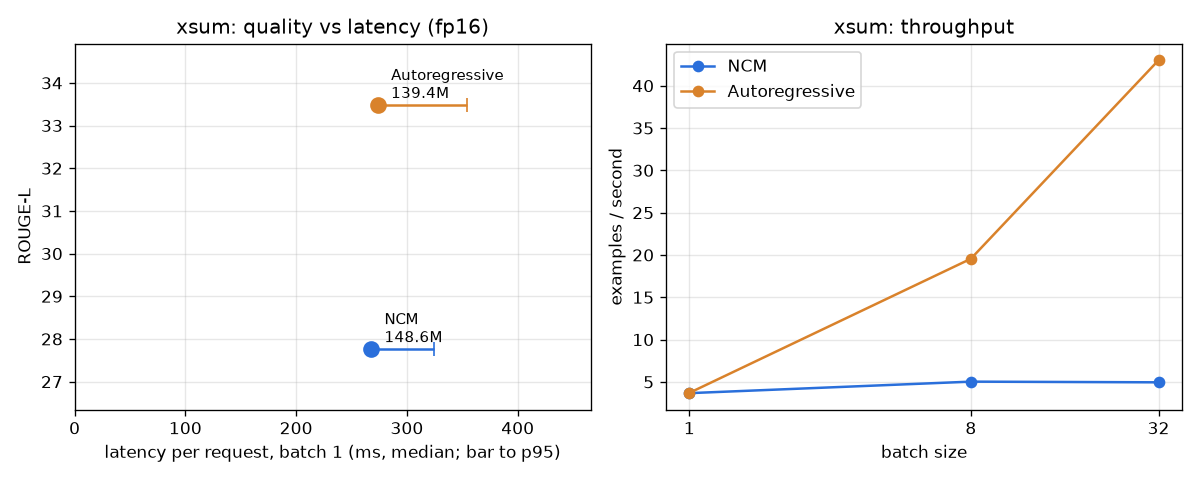
\includegraphics[width=\linewidth]{phase4_xsum_fp16.png}
\caption{XSum: quality vs.\ latency at batch 1 (left) and throughput vs.\ batch size (right).}
\label{fig:phase4}
\end{figure}

Table~\ref{tab:phase4} and Figure~\ref{fig:phase4} show the central result. At batch 1 NCM is as fast as BART on XSum
and 1.2$\times$ faster than opus-mt on WMT14, with a tighter p95 because its number of
passes does not depend on the output. At batch 32 the AR models are 2.3$\times$ (WMT14) to
8.7$\times$ (XSum) faster. Profiling explains why: each level pass re-runs the transformer
over the full input prefix (512 tokens for XSum, 9 times), with no KV cache in this
checkpoint's generation path, whereas BART encodes the article once and runs about 25 cheap
cached decoder steps. At batch 1 the GPU is under-used either way; at batch 32 NCM's
repeated prefix work dominates (7.6\,s of 8.0\,s per batch on XSum).

The quality gap mixes method and pretraining: both baselines start from large-scale
pretraining, while the NCM checkpoints are trained from scratch on the task data. The NCM
paper's matched-data AR baseline scores ROUGE-L 24.4 (NCM 28.0) and BLEU 25.2 (NCM 22.6).

\paragraph{What ``31$\times$'' means here.} The figure compares NCM's 8--11 passes with
128--184 diffusion steps on 1024-token outputs. Against an AR model with a KV cache, on
$\sim$20-word outputs, the step-count advantage mostly disappears.

\paragraph{Predictions vs.\ reality.} We predicted a 2--5$\times$ batch-1 speedup (wrong:
1.0--1.2$\times$), a shrinking advantage at larger batches (right, and it reverses), a larger
advantage on XSum (wrong: XSum is NCM's worst case), and higher memory use (right).

\section{NCM as a tool in RAG and agents}
\paragraph{Setup.} 40 XQuAD~\citep{xquad2020} questions over its 240 Wikipedia paragraphs,
MiniLM embeddings~\citep{sbert2019} with FAISS~\citep{faiss2019}, top-3 retrieval,
qwen2.5:3b answering. An answer is correct if a gold answer string appears in it.

\paragraph{Context compression.} Summarizing each retrieved paragraph before the LLM cuts
accuracy from 87.5\% to 10.0\% (NCM) and 17.5\% (BART) although retrieval still finds the
right paragraph 97.5\% of the time: a one-sentence news-style summary keeps the gist and
drops the fact the question asks for. It is also slower (809 vs.\ 423\,ms), because
compression costs more than the shorter prompt saves.

\paragraph{Multilingual RAG.} Translating the German version of the corpus (1,372 sentences)
with NCM gives 37.5\% accuracy vs.\ 67.5\% with opus-mt (English originals: 87.5\%), at
half the bulk speed (20 vs.\ 40 sentences/s at batch 32). NCM translations replace entity
names (``Luthers Schriften'' $\to$ ``Marx's writings''), which is fatal for retrieval.
\textbf{TODO:} these numbers used a sentence splitter that also split German ordinals
(``am 3.\ Oktober''); re-run with the fixed splitter and update.

\paragraph{Agent.} A hand-written tool-calling loop gives the LLM four tools: search and
three NCM models (summarize, translate, solve Sudoku). Over six multi-step tasks the LLM
accounts for 91--97\% of wall time and NCM tools for 3--9\%, so even an infinitely fast
NCM would barely change end-to-end latency. Prompt design mattered more than speed: with a
first prompt the LLM spent 28\,s and 1,449 tokens solving the Sudoku itself instead of calling the tool.

\section{Limits suite}\label{sec:limits}
Each experiment below pushes one axis until something breaks. Predictions are in
\texttt{docs/limits.md}, committed before running.

\subsection{Input length}
Inputs are $k$ consecutive WMT14 test sentences joined together, so length grows in a
controlled way and the reference stays exact; the AR model is allowed up to 400 output
tokens so its default cap is not what is measured.
\limitstable{input_length}{\texttt{python -m ncm\_lab.limits.run input-length}}
\limitsfig{input_length}{BLEU vs.\ input length on WMT14 De$\to$En.}{figure from
\texttt{input-length}}
\textbf{TODO:} interpretation.

\subsection{Batch size up to out-of-memory}
\limitstable{batch_sweep}{\texttt{python -m ncm\_lab.limits.run batch-sweep}}
\limitsfig{batch_sweep}{Throughput vs.\ batch size; markers end where the model runs out of
6\,GB.}{figure from \texttt{batch-sweep}}
\textbf{TODO:} interpretation (crossover batch size per task).

\subsection{Output length: where NCM's fixed step count pays off}
The AR model is forced to write exactly $L$ tokens and its latency is fitted as
$a + bL$; NCM's cost is constant up to its canvas size. The break-even $L^\ast = (t_\text{NCM}
- a)/b$ is NCM's speed niche on this GPU. This measures speed only: forced AR outputs are not
meaningful text, and NCM cannot write beyond its canvas.
\limitstable{output_length_breakeven}{\texttt{python -m ncm\_lab.limits.run output-length}}
\limitsfig{output_length}{Latency at batch 1 vs.\ output length.}{figure from
\texttt{output-length}}
\textbf{TODO:} interpretation.

\subsection{Faithfulness}
Abstractive summarizers are known to hallucinate~\citep{maynez2020}. We count outputs that
contain a number or a capitalized name absent from the source (for translation: absent from
source and reference), and outputs with a repeated word or bigram. These proxies over-count
equally for every model, so we compare models rather than read absolute rates.
\limitstable{faithfulness}{\texttt{python -m ncm\_lab.limits.run faithfulness} (CPU only)}
\textbf{TODO:} interpretation.

\subsection{Robustness to noisy input}
\limitstable{robustness}{\texttt{python -m ncm\_lab.limits.run robustness}}
\textbf{TODO:} interpretation.

\subsection{Sudoku out of distribution}
NCM vs.\ an exact backtracking solver and qwen2.5:3b on: the hard test set; the same puzzles
with digits relabelled and the grid transposed (logically identical); 5 or 15 clues removed
(any valid completion counts); unsolvable puzzles (a duplicate digit in a row, where the
right answer is to say so); and already-solved grids.
\limitstable{sudoku_stress}{\texttt{python -m ncm\_lab.limits.run sudoku-stress}}
\textbf{TODO:} interpretation.

\subsection{A specialist vs.\ a general LLM}
The same 100 examples per task through NCM, the AR baseline and zero-shot qwen2.5:3b, one
request at a time, end-to-end latency.
\limitstable{llm_vs_ncm}{\texttt{python -m ncm\_lab.limits.run llm-vs-ncm}}
\limitsfig{llm_vs_ncm}{Quality vs.\ median latency at batch 1.}{figure from
\texttt{llm-vs-ncm}}
\textbf{TODO:} interpretation.

\subsection{Agent reliability}
Each Phase 5 task runs 10 times at temperature 0.7 (and once at 0).
\limitstable{agent_reliability}{\texttt{python -m ncm\_lab.limits.run agent-reliability}}
\textbf{TODO:} interpretation.

\section{Discussion}
On a laptop GPU and short outputs, NCM's parallel decoding buys predictable single-request
latency, not throughput: its passes repeat work over the input prefix that an AR model with
a KV cache does once. Its speed would matter for long outputs (Section~\ref{sec:limits}),
against diffusion models, or with a cached prefix, none of which the released task
checkpoints exercise. As a tool in LLM pipelines, NCM's speed is dwarfed by the LLM, and
its weaknesses (lower quality than pretrained baselines, invented entities) are exactly the
ones RAG punishes.
\textbf{TODO:} update with the limits-suite findings.

\section{Limitations}
One GPU and one machine; results on an H100 or with larger batches may differ. Baselines are
pretrained while NCM checkpoints are not, so the quality gap is not only the method's.
Evaluation sets are small (500 examples per task, 40 RAG questions, six agent tasks):
enough to see large effects, not small ones. RAG accuracy uses lenient string containment.
fp16 is autocast with fp32 weights. We did not re-measure the diffusion baseline behind the
31$\times$ claim. Faithfulness uses string proxies, not human judgment.

\section{Reproducibility}
Code, configuration, every output and per-example log are at
\url{https://github.com/Aymenrahmanii/NCM}. \texttt{bash scripts/reproduce\_results.sh}
recreates every number; the service, tests and CI run without a GPU using stand-in models.

\section*{Use of AI assistance}
\textbf{TODO, keep and adapt:} Parts of the code, documentation and a first draft of this
paper were written with the help of an AI assistant (Claude, Anthropic). All experiments
were run, and all results checked, by the author, who takes full responsibility for the
content.

\bibliographystyle{plainnat}
\bibliography{refs}
\end{document}
